\documentclass[tikz,border=20pt]{standalone}
\usepackage{mathptmx}
\usepackage{tikz}
\usetikzlibrary{arrows.meta, calc, positioning}

\tikzset{
  extentity/.style={rectangle, draw=black, line width=1.5pt,
    minimum width=2.6cm, minimum height=0.8cm,
    font=\bfseries\small, align=center},
  process/.style={circle, draw=black, line width=1.2pt,
    minimum size=2.4cm, font=\small, align=center},
  datastore/.style={rectangle, draw=black, line width=1pt,
    minimum width=3.2cm, minimum height=0.7cm,
    font=\small, align=center,
    append after command={
      \pgfextra{
        \draw[line width=1pt] (\tikzlastnode.north west) -- (\tikzlastnode.north east);
        \draw[line width=1pt] (\tikzlastnode.south west) -- (\tikzlastnode.south east);
      }
    }
  },
  flow/.style={->, >=Stealth, line width=0.8pt},
  flabel/.style={font=\fontsize{7}{8}\selectfont, align=center,
    fill=white, inner sep=1pt, text width=1.8cm}
}

\begin{document}
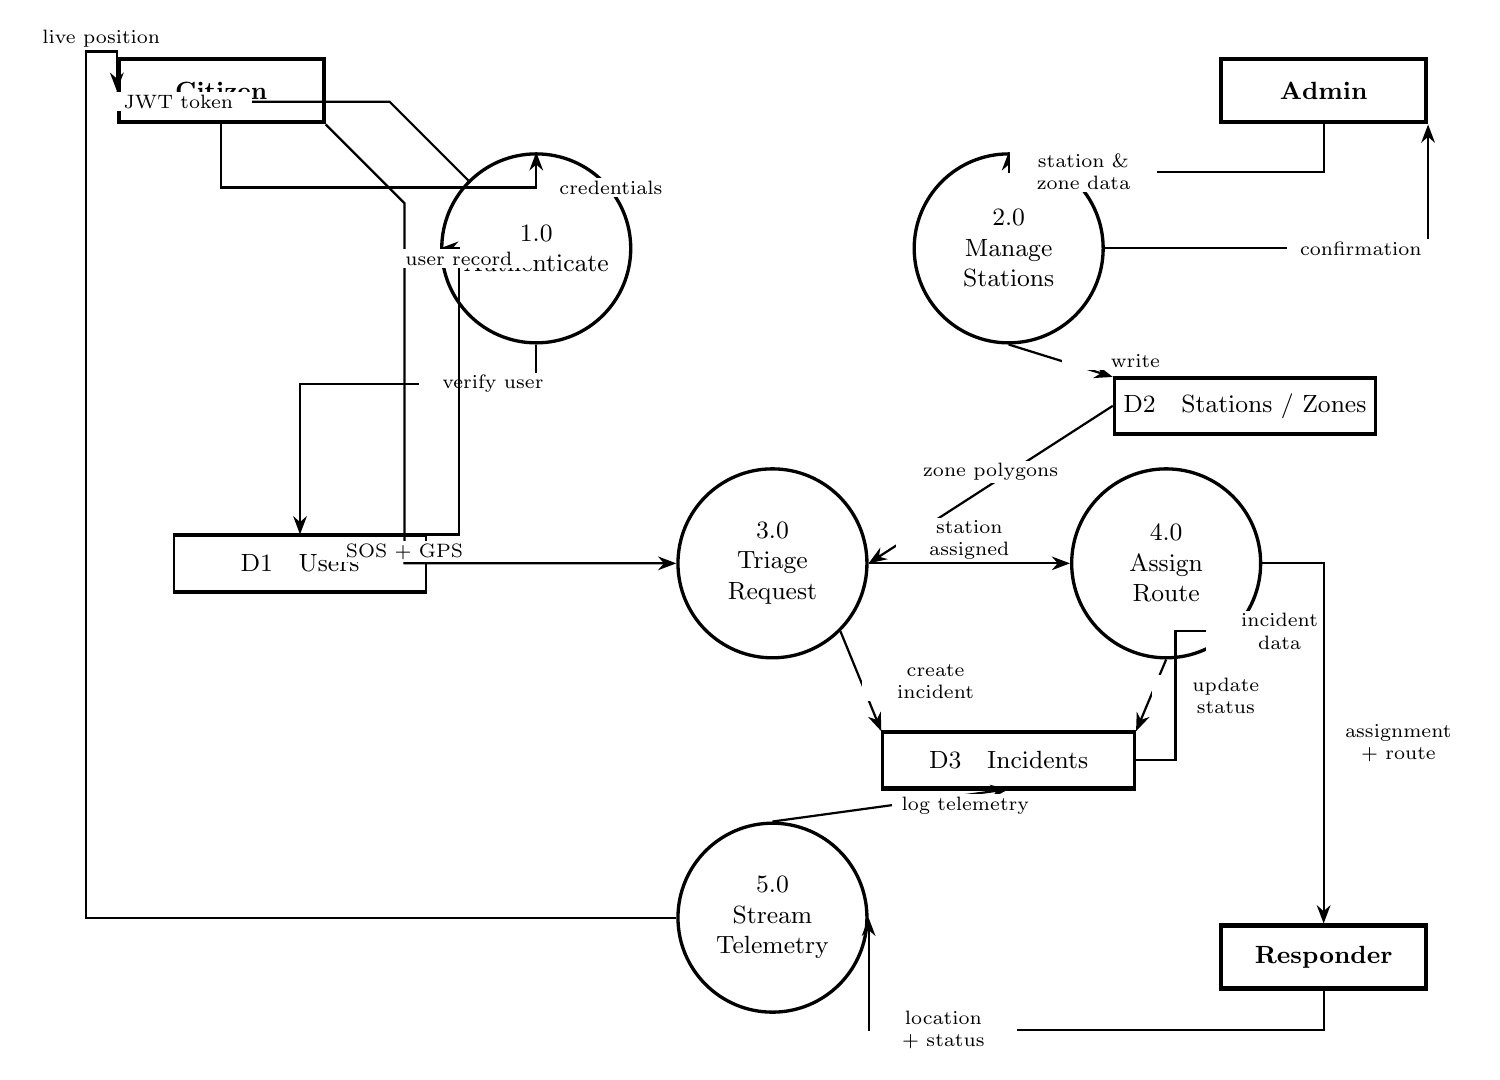
\begin{tikzpicture}

%% External entities
\node[extentity] (citizen)   at (-7,  6)  {Citizen};
\node[extentity] (admin)     at ( 7,  6)  {Admin};
\node[extentity] (responder) at ( 7, -5)  {Responder};

%% Processes
\node[process] (p1) at (-3,  4)   {1.0\\Authenticate};
\node[process] (p2) at ( 3,  4)   {2.0\\Manage\\Stations};
\node[process] (p3) at ( 0,  0)   {3.0\\Triage\\Request};
\node[process] (p4) at ( 5,  0)   {4.0\\Assign\\Route};
\node[process] (p5) at ( 0, -4.5) {5.0\\Stream\\Telemetry};

%% Data stores
\node[datastore] (d1) at (-6,  0)  {D1\quad Users};
\node[datastore] (d2) at ( 6,  2)  {D2\quad Stations / Zones};
\node[datastore] (d3) at ( 3, -2.5){D3\quad Incidents};

%% ── Citizen → 1.0 Authenticate
\draw[flow] (citizen.south) -- ++(0,-0.8) -| (p1.north)
  node[flabel, midway, right] {credentials};
\draw[flow] (p1.north west) -- ++(-1,1) -| (citizen.west)
  node[flabel, near start, left] {JWT token};

%% ── Admin → 2.0 Manage Stations
\draw[flow] (admin.south) -- ++(0,-0.6) -| (p2.north)
  node[flabel, midway, right] {station \& zone data};
\draw[flow] (p2.east) -- ++(0.5,0) -| (admin.south east)
  node[flabel, near start, right] {confirmation};

%% ── Citizen → 3.0 Triage Request
\draw[flow] (citizen.south east) -- ++(1,-1) |- (p3.west)
  node[flabel, midway, above] {SOS + GPS};

%% ── 1.0 ↔ D1 Users
\draw[flow] (p1.south) -- ++(0,-0.5) -| (d1.north)
  node[flabel, near start, right] {verify user};
\draw[flow] (d1.north east) -- ++(0.4,0) |- (p1.west)
  node[flabel, midway, below] {user record};

%% ── 2.0 ↔ D2 Stations/Zones
\draw[flow] (p2.south) -- (d2.north west)
  node[flabel, midway, right] {write};
\draw[flow] (d2.west) -- (p3.east)
  node[flabel, midway, above] {zone polygons};

%% ── 3.0 → D3 Incidents
\draw[flow] (p3.south east) -- (d3.north west)
  node[flabel, midway, right] {create incident};

%% ── 3.0 → 4.0 Assign Route
\draw[flow] (p3.east) -- (p4.west)
  node[flabel, midway, above] {station\\ assigned};

%% ── 4.0 ↔ D3 Incidents
\draw[flow] (p4.south) -- (d3.north east)
  node[flabel, midway, right] {update\\ status};
\draw[flow] (d3.east) -- ++(0.5,0) |- (p4.south east)
  node[flabel, near end, right] {incident\\ data};

%% ── 4.0 → Responder
\draw[flow] (p4.east) -- ++(0.4,0) -| (responder.north)
  node[flabel, near end, right] {assignment\\ + route};

%% ── Responder → 5.0 Stream Telemetry
\draw[flow] (responder.south) -- ++(0,-0.5) -| (p5.east)
  node[flabel, midway, right] {location\\ + status};

%% ── 5.0 → D3 Incidents
\draw[flow] (p5.north) -- (d3.south)
  node[flabel, midway, right] {log telemetry};

%% ── 5.0 → Citizen (live tracking)
\draw[flow] (p5.west) -- ++(-7.5,0) -- ++(0,11) -| (citizen.west)
  node[flabel, near start, above] {live position};

\end{tikzpicture}
\end{document}
